%!TEX root = draft.tex
\vspace{-3.5mm}
\section{Stacks With Fixed Pop Commit Points}\label{sec:stacks}
\vspace{-1.5mm}
The abstract implementation in Section~\ref{sec:queues} can be adapted to stacks, the main modification being that the linearization point $lin(pop,d,k)$ with $d\neq{\tt EMPTY}$ is enabled when $k$ is added by a push which is maximal in the happens-before order stored in the state. However, there are stack implementations, e.g., Time-Stamped Stack~\cite{DBLP:conf/popl/DoddsHK15} ($\mathit{TSS}$, for short), which cannot be proved correct using forward simulations to this abstract implementation because the linearization points of the pop operations are not fixed.
%this stack implementation cannot simulate (through forward simulations) existing stack implementations like the Time-Stamped Stack~\cite{DBLP:conf/popl/DoddsHK15} ($\mathit{TSS}$, for short) where the linearization points of the pop operations are not fixed. 
Exploiting particular properties of the stack semantics, we refine the ideas used in $AbsQ$ and define 
a new abstract implementation for stacks, denoted as $AbsS$, which is able to simulate such implementations. Forward simulations to $AbsS$ are complete for proving the correctness of stack implementations provided that the point in time where the return value of a pop operation is determined, called \emph{commit point}, corresponds to a fixed statement in the pop method.
% provided that the point in time where the return value of a pop operation is determined corresponds to a fixed action. To demonstrate the use of this abstract implementation we provide a correctness proof for a simplified version of Time-Stamped Stack that preserves its most complex behaviors.

\vspace{-3.5mm}
\subsection{Pop Methods With Fixed Commit Points}
\vspace{-1mm}
\begin{wrapfigure}{l}{5.2cm}
\vspace{-10.5mm}
\begin{lstlisting}
struct Node{
  int data;
  int ts;
  Node* next;
  boolean taken;
};
Node* pools[maxThreads];
int TS = 0;   

void push(int x) {
  Node* n = new Node(x,MAX_INT,
                        null,false);
  n->next = pools[myTID];
  pools[myTID] = n;
  int i = TS++;
  n->ts = i;
}
int pop() {
 boolean success = false;
 int maxTS = -1;
 Node* youngest = null;
 while ( !success ) {
   maxTS = -1; youngest = null;
   for(int i=0; i<maxThreads; i++){
     Node* n = pools[i];
     while (n->taken && n->next != n)
       n = n->next;
     if(maxTS < n->ts) {
       maxTS = n->ts; youngest = n;
     }
   }
   if (youngest != null)
     success=CAS(youngest->taken,
                       false,true);
 }
 return youngest->data;
}
\end{lstlisting}
\vspace{-6mm}
\caption{Time-Stamped Stack.} %We assume that every statement is atomic.}
\label{fig:TimeStamped}
\vspace{-7mm}
\end{wrapfigure}
We explain the meaning of the commit points on a simplified version of the Time-Stamped Stack~\cite{DBLP:conf/popl/DoddsHK15} ($\mathit{TSS}$, for short) given in Fig.~\ref{fig:TimeStamped}. This  implementation maintains an array of singly-linked lists, one for each thread, where list nodes contain a data value (field {\tt data}), a timestamp (field {\tt ts}), the next pointer (field {\tt next}), and a boolean flag indicating whether the node represents a value removed from the stack (field {\tt taken}). Initially, each list contains a sentinel dummy node pointing to itself with timestamp $-1$ and the flag {\tt taken} set to {\tt false}.

Pushing a value to the stack proceeds in several steps: adding a node with maximal timestamp in the list associated to the thread executing the push (given by the special variable {\tt myTID}), asking for a new timestamp (given by the shared variable {\tt TS}), and updating the timestamp of the added node. Popping a value from the stack consists in traversing all the lists, finding the first element which doesn't represent a removed value (i.e., {\tt taken} is {\tt false}) in each list, and selecting the element with the maximal timestamp. A compare-and-swap (CAS) is used to set the {\tt taken} flag of this element to {\tt true}. The procedure restarts if the CAS fails.

\begin{figure}[t]
\centering
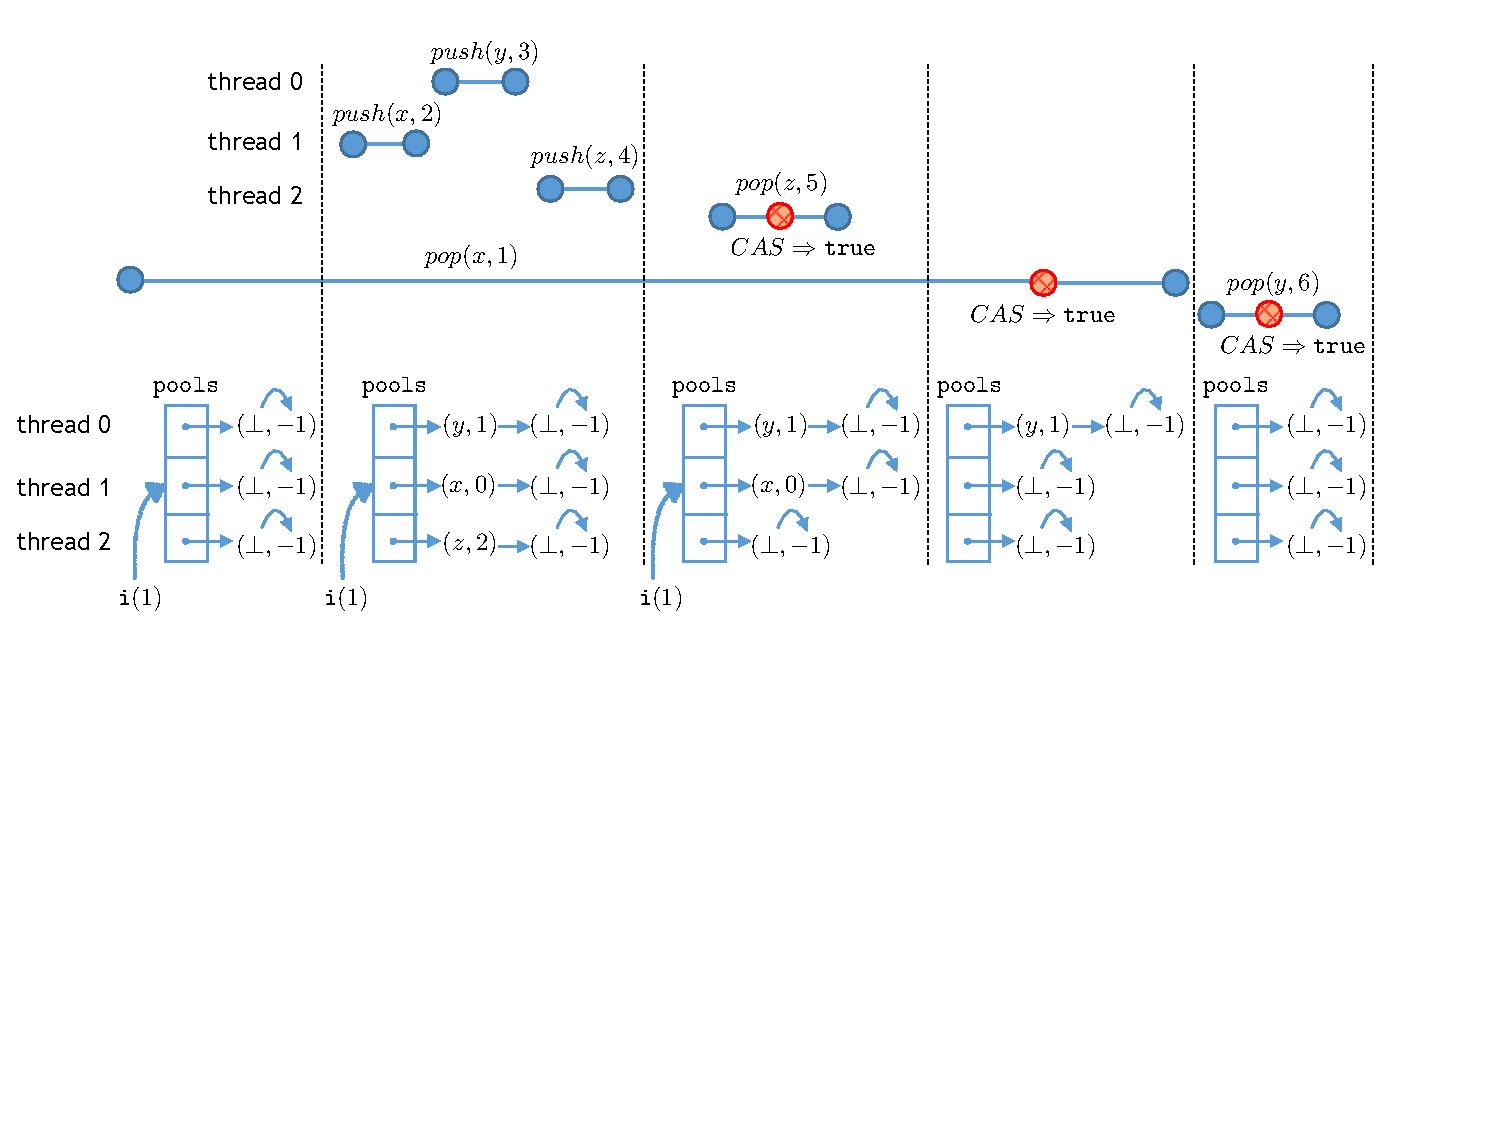
\includegraphics[width=11.5cm]{fig-tss.pdf}
\vspace{-4mm}
\caption{An execution of $\mathit{TSS}$. An operation is pictured by a line delimited by two circles denoting the call and respectively, the return action. Pop operations with identifier $k$ and removing value $d$ are labeled $pop(d,k)$. Their representation includes another circle that stands for a successful CAS which is their commit point. The library state after an execution prefix delimited at the right by a dotted line is pictured in the bottom part (the picture immediately to the left of the dotted line). A pair $(d,t)$ represents a list node with ${\tt data}=d$ and ${\tt ts}=t$, and ${\tt i}(1)$ denotes the value of {\tt i} in the pop with identifier 1. We omit the nodes where the field {\tt taken} is {\tt true}.}
\label{fig:commit}
\vspace{-6mm}
\end{figure}


The push operations don't have a fixed linearization point because adding a node to a list and updating its timestamp are not executed in a single atomic step. The nodes can be added in an order which is not consistent with the order between the timestamps assigned later in the execution. Also, the value added by a push that just added an element to a list can be popped before the value added by a completed push (since it has a maximal timestamp). The same holds for pop operations: The only reasonable choice for a linearization point is a successful CAS (that results in updating the field {\tt taken}). Fig.~\ref{fig:commit} pictures an execution showing that this action doesn't correspond to a linearization point, i.e., an execution for which the pop operations in every correct linearization are not ordered according to the order between successful CASs. In every correct linearization of that execution, the pop operation removing $x$ is ordered before the one removing $z$ although they perform a successful CAS in the opposite order.

An interesting property of the successful CASs in pop operations is that they fix the return value, i.e., the return value is {\tt youngest->data} where {\tt youngest} is the node updated by the CAS. We call such actions \emph{commit points}. More generally, commit points are actions that access shared variables, from which every control-flow path leads to the return control point and contains no more accesses to the shared memory (i.e., after a commit point, the return value is computed using only local variables).

%The complete version of $\mathit{TSS}$~\cite{DBLP:conf/popl/DoddsHK15} contains also a mechanism for elimination (a pop can remove a value without traversing all the lists if it has been added by a concurrent push) and emptiness checking. In both cases, the commit points can be identified in the code and correspond to certain boolean conditions evaluated to {\tt true}.

%TODO WHAT CAN WE SAY ABOUT COMMIT POINTS IN OTHER IMPLEMENTATIONS

%Usually, a stack implementation stores the pushed values into a data structure, e.g., a singly-linked list, and a pop operation contains an action (typically, a compare-and-swap) that removes an element from this data structure (or sets a flag associated to this element to a ``deleted'' state). Such an action represents a commit point since the pop operation will return the value stored in this element. 


%TODO GIVE AN EXAMPLE TO SHOW THE ISSUE WITH POP LINEARIZATION POINTS, AND TO SHOW THAT COMMIT POINTS ARE RIGHT LIMITS FOR THE INTERVAL OF A LIN POINT, I.E., A POP WITH A LATER COMMIT POINT CAN BE LINEARIZED BEFORE. NEED ONLY 2 POPS IN AN EXECUTION 

When the commit points of pop operations are fixed to particular implementation actions (e.g., a successful CAS) we assume that the library is an LTS over an alphabet that contains actions $com(pop,d,k)$ with $d\in\<Vals>$ and $k\in\<Ops>$ (denoting the commit point of the pop with identifier $k$ and returning $d$). Let $Com(pop)$ be the set of such actions.
%We consider a set of actions $Com(pop)=\set{com(pop,d,k):d\in\<Vals>, k\in\<Ops>}$, called \emph{commit points}, representing actions of a pop operation where its return value is determined. 
%TODO DESCRIBE THE TIME-STAMPED STACK, EXPLAIN THAT NO METHOD HAS A FIXED LIN POINT, GIVE THE COMMIT POINTS, SHOW THAT COMMIT POINTS ARE NOT LIN POINTS
%
%COMMIT POINTS ARE LINEARIZATION POINTS WHEN THE LIBRARY IS INTERPRETED AS A MULTISET

\vspace{-3mm}
\subsection{Abstract stack implementation}
\vspace{-1mm}
We define an abstract stack $AbsS$ over alphabet $C\cup R\cup Com(pop)$ that essentially, similarly to $AbsQ$, maintains the happens-before order of the pushes whose value has not yet been  removed by a matching pop. Pop operations are treated differently since the commit points are not necessarily linearization points. Intuitively, a pop can be linearized before its commit point. Each pop operation starts by taking a snapshot of the completed push operations which are maximal in the happens-before, more precisely, which don't happen before another completed push operation. Also, the library maintains the set of push operations overlapping with each pop operation. The commit point $com(pop,d,k)$ with $d\neq {\tt EMPTY}$ is enabled if either $d$ was added by one of the push operations in the initial snapshot, or by a push happening earlier when arguments of pushes from the initial snapshot have been removed, or by one of the push operations that overlaps with pop $k$. The commit point $com(pop,{\tt EMPTY},k)$ is enabled if all the values added by push operations happening before $k$ have been removed. The effect of the commit points is explained below through examples.
\vspace{-.4mm}

%\begin{wrapfigure}{l}{7.8cm}
%\vspace{-6mm}
\begin{figure}[t]
\centering
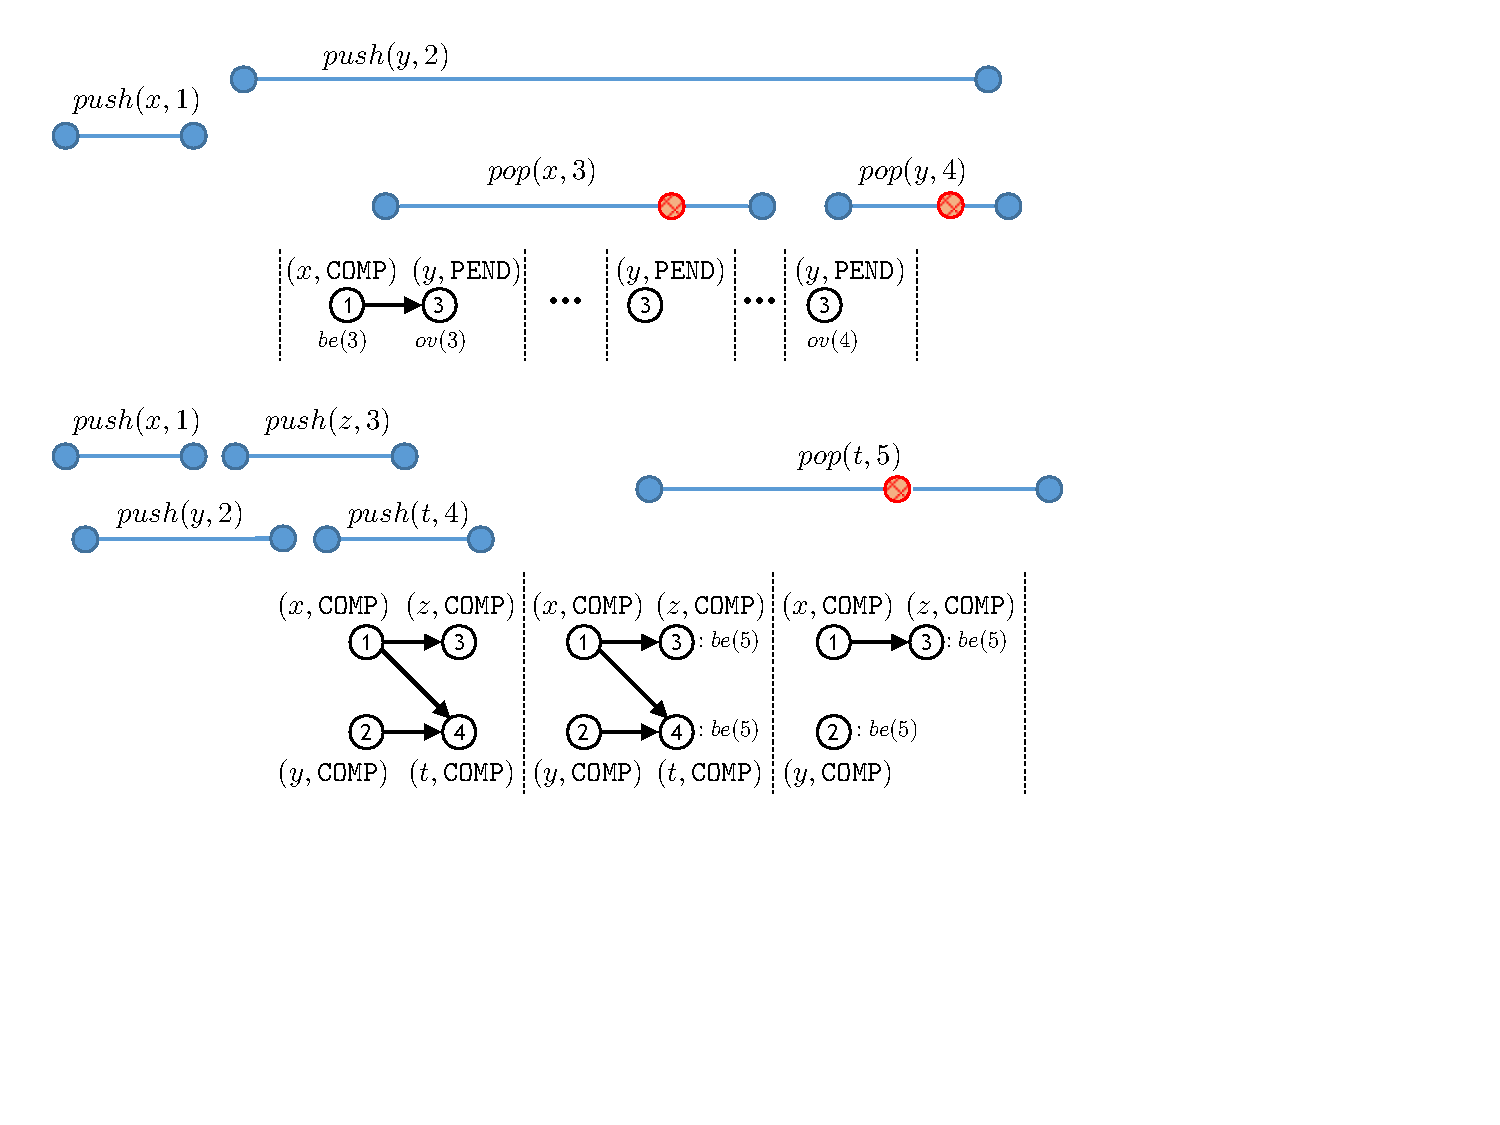
\includegraphics[width=10cm]{fig-stack.pdf}
%
%\vspace{2mm}
%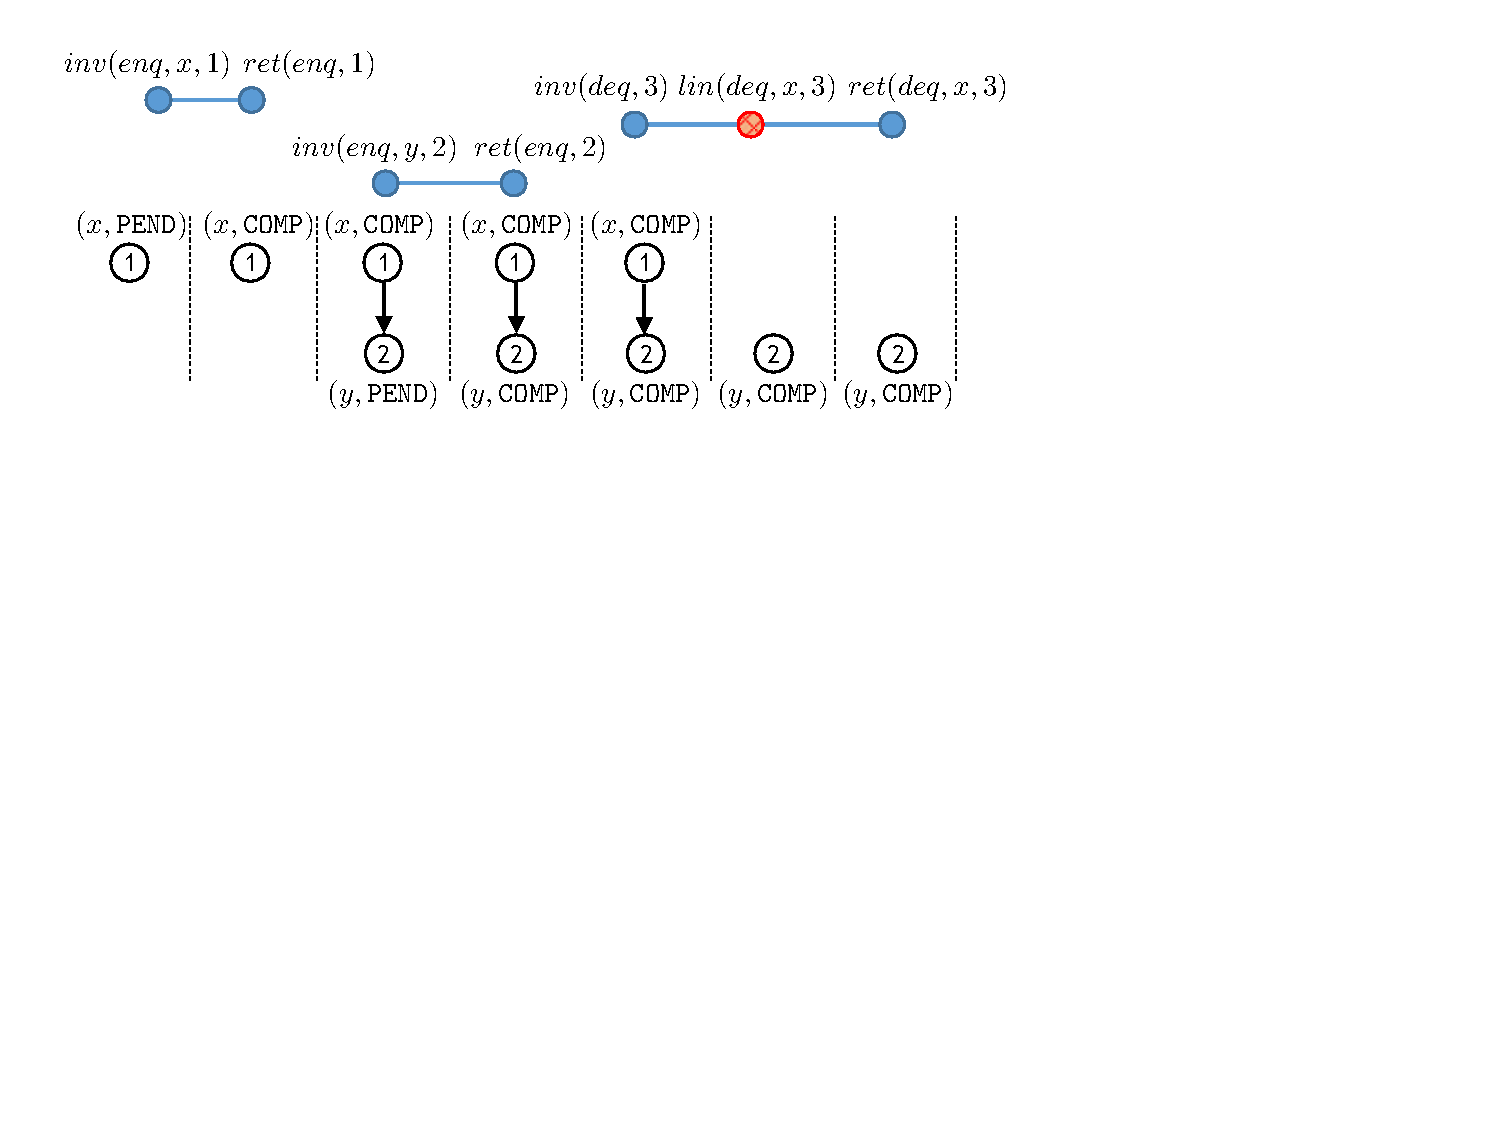
\includegraphics[width=7cm]{fig-queue2.pdf}
\vspace{-2mm}
\caption{Simulating stack histories with $AbsS$.}
\label{fig:stackSim}
\vspace{-6.5mm}
\end{figure}

Fig.~\ref{fig:stackSim} pictures two executions of $AbsS$ for two extended histories (that include pop commit points). For readability, we give the state of $AbsS$ only after several execution prefixes delimited at the right by a dotted line. We focus on pop operations -- the effect of push calls and returns is similar to enqueue calls and returns in $AbsQ$. Let us first consider the history on the top part. The first state we give is reached after the call of pop with identifier $3$. This shows the effect of a pop invocation: the greatest completed pushes according to the current happens-before (here, the push with identifier $1$) are marked as $be(3)$ (from ``before'' operation 3), and the pending pushes are marked as $ov(3)$ (from ``overlapping'' with operation 3). As a side remark, any other push operation that starts after pop $3$ would be also marked as $ov(3)$.
The commit point $com(pop,x,3)$ (pictured with a red circle) is enabled because $x$ was added by a push marked as $be(3)$. The effect of the commit point is that push $1$ is removed from the state (the execution on the bottom shows a more complicated case). For the second pop, the commit point $com(pop,y,4)$ is enabled because $y$ was added by a push marked as $ov(4)$. The execution on the bottom shows an example where the marking $be(k)$ for some pop $k$ is updated at commit points. The pushes $3$ and $4$ are marked as $be(5)$ and $be(6)$
when the pops $5$ and $6$ start. Then, $com(pop,t,5)$ is enabled since $t$ was added by $push(t,4)$ which is marked as $be(5)$. Besides removing $push(t,4)$, the commit point produces a state where a pop committing later, e.g., pop $6$, can remove $y$ which was added by a predecessor of $push(t,4)$ in the happens-before ($y$ could become the top of the stack when $t$ is removed). This history is valid because $push(y,2)$ can be linearized after $push(x,1)$ and $push(z,3)$. Thus, push 2, a predecessor of the push which is removed, is marked as $be(6)$. Push $1$ which is also a predecessor of the removed push is not marked as $be(6)$ because it happens before another push, i.e., push 3, which is already marked as $be(6)$ (the value added by push 3 should be removed before the value added by push 1 could become the top of the stack).

\begin{figure} [t]
%\vspace{-2mm}
\hspace{-15mm}
\begin{minipage}[t]{7.5cm}
\scriptsize{
{	%\centering
	\begin{align*}
%		& \mathsf{Operations}, \mathsf{Values} : \mathsf{Sort} \\
		& \text{\underline{Shared State}} \\
		& \text{{\ttfamily \bfseries function}}\ \mathsf{present} : \<Ops> \rightarrow \{{\tt true},{\tt false}\} \\
		& \text{{\ttfamily \bfseries function}}\ \mathsf{pending} : \<Ops> \rightarrow \{{\tt true},{\tt false}\} \\
		& \text{{\ttfamily \bfseries function}}\ \mathsf{arg} : \<Ops> \rightarrow \mathsf{Values} \\
		& \text{{\ttfamily \bfseries function}}\ \mathsf{before} : \<Ops> \times \<Ops> \rightarrow \{{\tt true},{\tt false}\} \\
		& \text{{\ttfamily \bfseries function}}\ \mathsf{maxAtInvoc} : \<Ops> \rightarrow 2^{\<Ops>} \\
		& \text{{\ttfamily \bfseries function}}\ \mathsf{overlap} : \<Ops> \rightarrow 2^{\<Ops>} \\
%		& \mathsf{stored}, \mathsf{pending} : \mathsf{Operations} &\mbox{ // the status of an enqueue} \\
%		& \mathsf{arg} : \mathsf{Operations} \rightarrow \mathsf{Values} &\mbox{ // the argument of an enqueue} \\
	\end{align*}
}}
\end{minipage}
\begin{minipage}[t]{7.3cm}
\begin{lstlisting}
void push($\<Vals>$ x) {
  atomic rule inv(push,x,k = new);
  atomic rule ret(push,k);
}

$\<Vals>$ pop() {
  atomic rule inv(pop,k = new);
  atomic rule com(pop,y,k);
  atomic rule ret(pop,y,k);
}
\end{lstlisting}
\end{minipage}

\vspace{-5mm}
\begin{minipage}[t]{6.2cm}
\begin{lstlisting}
rule inv(push,x,k) = {
  $\mathsf{present}$(k) = true;
  $\mathsf{pending}$(k) = true;
  $\mathsf{arg}$(k) = x;
  forall k1 with $\mathsf{present}$(k1)$\land \neg \mathsf{pending}$(k1) do
    $\mathsf{before}$(k1,k) = true;
  forall k1 do
    $\mathsf{overlap}$(k1) = $\mathsf{overlap}$(k1) $\cup$ $\{$k$\}$;
}
rule ret(push,k) = {
  $\mathsf{pending}$(k) = false;
  return;
}
\end{lstlisting}
\end{minipage}
\begin{minipage}[t]{5cm}
%\vspace{-3mm}
\begin{lstlisting}
rule inv(pop,k) = {
  forall k1 with $\mathsf{present}$(k1)$\land \neg \mathsf{pending}$(k1)$\land$
                 $\neg \exists k'.\ \mathsf{present}(k')\land \neg \mathsf{pending}(k')\,\land$ 
                 $\mathsf{before}$(k1,$k'$) do
    $\mathsf{maxAtInvoc}$(k) = $\mathsf{maxAtInvoc}$(k) $\cup$ $\{$k1$\}$;
  forall k1 with $\mathsf{present}$(k1)$\land \mathsf{pending}$(k1) do
    $\mathsf{overlap}$(k) = $\mathsf{overlap}$(k) $\cup$ $\{$k1$\}$;
}
rule ret(pop,y,k) = {
  return y;
}
\end{lstlisting}
\end{minipage}

\vspace{-4mm}
\begin{lstlisting}
rule com(pop,y,k) = {
  choose a $\in$ {true, false};
  if ((a || $\forall k'.\ \mathsf{present}(k')$=false) && $\mathsf{maxAtInvoc}$(k)=$\,\emptyset$) 
    y = EMPTY;
  else 
    choose k1 $\in\<Ops>$ with $\mathsf{present}$(k1)$\land$ k1$\in\mathsf{maxAtInvoc}$(k)$\cup\,\mathsf{overlap}$(k) do
    $\mathsf{present}$(k1) = false;
    y = $\mathsf{arg}$(k1);
    forall k2 with k1$\in\mathsf{maxAtInvoc}$(k2) do
      $\mathsf{maxAtInvoc}$(k2) = $\mathsf{maxAtInvoc}$(k2)$\setminus\{$k1$\}$;
      forall k3 with $\mathsf{before_1}$(k3,k1)$\land \forall k'.\ (\mathsf{before_1}($k3$,k')\land k'\neq $k1$)\Rightarrow k'\in \mathsf{overlap}($k2$)$ do
        $\mathsf{maxAtInvoc}$(k2) = $\mathsf{maxAtInvoc}$(k2)$\cup\{$k3$\}$;
}
\end{lstlisting}
 %\neg\exists k'.\ \mathsf{present}(k')\,=\,$true$\,\land\, \mathsf{before}($k3,$k')\land \mathsf{before}(k',$k1$)$

%{\scriptsize
%  \centering
%  \begin{mathpar}
%    \inferrule[call-push]{
%      k\not\in dom(cp) \\ 
%      d\neq {\tt EMPTY} \\
%      \forall k'.\ ov'(k') = ov(k')\cup \{k\}
%    }{
%      O,<,\ell,rv,cp,be,ov 
%      \xrightarrow{inv(push,d,k)} 
%      O\cup\{k\},<\cup\ {\tt COMP}(O)\times\{k\},\ell[k\mapsto (d,{\tt PEND})],rv,cp[k\mapsto A_1],be,ov'
%    }\hspace{5mm}
%
%    \vspace{-1mm}
%    \inferrule[call-pop]{
%      k\not\in dom(cp) %\\ k\not\in dom(cp) \\ k\not\in dom(cp)
%    }{
%      O,<,\ell,rv,cp,be,ov
%      \xrightarrow{inv(pop,k)} 
%      O,<,\ell,rv,cp[k\mapsto R_1],be[k\mapsto maxCo(O)],ov[k\mapsto {\tt PEND}(O)]
%    }\hspace{5mm}
%    
%    \vspace{-1mm}
%    \inferrule[ret-pop]{
%       cp(k) = R_2 \\
%       rv(k)=d  
%    }{
%      O,<,\ell,rv,cp,be,ov
%      \xrightarrow{ret(pop,d,k)}
%      O,<,\ell,rv,cp[k\mapsto R_3],be,ov
%    }\hspace{5mm}
%
%    \vspace{-1mm}
%    \inferrule[ret-push1]{
%      cp(k) = A_1 \\
%      k \in O \\
%      \ell(k) = (d,{\tt PEND}) 
%    }{
%      O,<,\ell,rv,cp,be,ov
%      \xrightarrow{ret(push,k)}
%      O,<,\ell[k\mapsto (d,{\tt COMP})],rv,cp[k\mapsto A_2],be,ov
%    }\hspace{5mm}
%    \inferrule[ret-push2]{
%      cp(k) = A_1 \\
%      k \not\in O 
%    }{
%      O,<,\ell,rv,cp,be,ov
%      \xrightarrow{ret(push,k)}
%      O,<,\ell,rv,cp[k\mapsto A_2],be,ov
%    }\hspace{5mm}
%
%    \inferrule[com-pop1]{
%       cp(k) = R_1 \\
%       d\neq{\tt EMPTY} \\
%       k'\in be(k)\cup ov(k) \\
%        \ell_1(k')=d \\
%       \forall k_1.\ k'\not\in be(k_1) \Rightarrow be'(k_1)=be(k_1) \\     \\
%       \forall k_1.\ k'\in be(k_1) \Rightarrow be'(k_1)=(be(k_1)\setminus\{k'\})\cup \{k_2: k_2\in pred_{<}(k') \land \forall k_3. (k_2\in pred_{<}(k_3) \land k_3\neq k') => k_3\in ov(k_1)\} \\
%    }{
%      O,<,\ell,rv,cp,be,ov
%      \xrightarrow{com(pop,d,k)} \\
%      O\setminus \{k'\},<\uparrow k',\ell,rv[k\mapsto d],cp[k\mapsto R_2],be',ov %be[\forall k''.\ k'\in be(k'') \Rightarrow k'' \mapsto (be(k'')\cup pred_{<}(k'))\setminus\{k'\}]
%    }\hspace{5mm}
%
%    %\vspace{-1mm}
%    \inferrule[com-pop2]{
%       cp(k) = R_1 \\
%       be(k)=\emptyset
%    }{
%      O,<,\ell,rv,cp,be,ov
%      \xrightarrow{com(pop,{\tt EMPTY},k)}
%      O,<,\ell,rv[k\mapsto {\tt EMPTY}],cp[k\mapsto R_2],be,ov
%    }\hspace{5mm}
%
%    
%      \end{mathpar}
%  }
 \vspace{-4mm}
  \caption{The abstract stack implementation $AbsS$. We use $\mathsf{before_1}$ to denote the immediate successor relation induced by $\mathsf{before}$, i.e., $\mathsf{before}_1(k,k')={\tt true}$ iff $\neg\exists k''.\ \mathsf{present}(k'')\land \mathsf{before}(k,k'')\land \mathsf{before}(k'',k')$.
%  The transition relation of $AbsQ$. We use the following notions: $maxCo(O)$ is the set of greatest operations in $O$ (w.r.t. $<$) which are completed, i.e., $maxCo(O)=\set{k\in O: \ell_2(k)={\tt COMP}, \forall k'\in O.\ k' < k \vee \ell_2(k')={\tt PEND}}$, ${\tt PEND}(O)=\{k\in O: \ell_2(k)={\tt PEND}\}$, and $pred_{<}(k')$ is the set of immediate predecessors of $k'$ according to $<$, i.e., $pred_{<}(k')=\set{k\in O: k < k'\land \forall k''\in O.\ k'' > k' \vee k'' < k}$.%\textcolor{red}{call-push should have $d \neq EMPTY$ in the premise. If I understand correctly, there is a problem change in $be$ in lin-pop1 rule. What I understand is we move $k''$ to every predecesoor of $k'$. But we should not move it to predecessor of $k'$ if this predecessor has a successor $m$ such that $m \in be(k'')$. Is this case reflected in your definition. Please read sub-bullet 4 of bullet 4 in the definition of $L_I$ in my document. Lin-pop2 seems ok for me. Last note: Bibliography seems not correct to me.}  $f[\forall k.\ k\mapsto expr(k)]$ is the function $g$ defined by $g(k)=expr(k)$,   $g(k)=f(k)$ for all $k$ such that $guard(k)$ is false, and 
  }
  \label{fig:transitions:AbsS}
\vspace{-5mm}
\end{figure}

The description of $AbsS$ as an abstract state machine is given in Fig.~\ref{fig:transitions:AbsS}. Compared to the queue implementation $AbsQ$, the shared state contains two more functions $\mathsf{maxAtInvoc}$ and $\mathsf{overlap}$. For each pop operation $k$, $\mathsf{maxAtInvoc}(k)$ records the set of completed push operations which were maximal in the happens-before (defined by $\mathsf{before}$) when pop $k$ was invoked, or happening earlier provided that the values of all the pushes happening later than one of these maximal ones have been removed. Also, for each pop operation $k$, $\mathsf{overlap}(k)$ contains the push operations overlapping with pop $k$.
%Formally, the states of $AbsS$ are tuples $\tup{O,<,\ell,rv,cp,be,ov}$ where $<$ is a strict partial order over the set $O$ of operation identifiers, $\ell: O -> \<Vals>\times\{\tt{PEND,\tt{COMP}}\}$ labels every identifier in $O$ with a value and a pending/completed flag, $rv:\<Ops> ~> \<Vals>$ records the return value of a pending pop fixed at its commit point, $cp:\<Ops> ~> \{A_1,A_2,R_1,R_2,R_3\}$ records the control point of every push ($A_1, A_2$) or pop operation ($R_1,R_2,R_3$), $be:\<Ops> ~> 2^O$ records the greatest completed push operations before a pop started or happening earlier provided that the values of all the push happening later have been removed, and $ov: \<Ops> ~> 2^O$ records push operations overlapping with a pop.
%%The initial state has all these components set to $\emptyset$ and the transition relation $->$ is defined in Figure~\ref{fig:transitions:AbsS}.
%All the components are $\emptyset$ in the initial state, and the transition relation $->$ is defined in Fig.~\ref{fig:transitions:AbsS}.
In the initial state, the domain of every function (predicate) is empty. The push methods are similar to the enqueue methods in $AbsQ$. The only difference is that every newly invoked push operation {\tt k} is added to the set $\mathsf{overlap}(${\tt k1}$)$ for all pop operations {\tt k1} (since {\tt k} overlaps with all the currently pending pops). The rule {\tt inv(pop,k)}, marking the invocation of a pop, sets $\mathsf{maxAtInvoc}(${\tt k}$)$ and $\mathsf{overlap}(${\tt k}$)$ as explained above. The rule {\tt com(pop,y,k)} results in setting the return value {\tt y} to {\tt EMPTY} if the set $\mathsf{maxAtInvoc}(${\tt k}$)$ is empty (otherwise, there would be push operations happening before pop {\tt k} which makes the answer {\tt EMPTY} incorrect). It results in setting the return value to a value $d\neq\,${\tt EMPTY} when $d$ was added by a push {\tt k1} which belongs to $\mathsf{maxAtInvoc}(${\tt k}$)$ or $\mathsf{overlap}(${\tt k}$)$. In this latter case, the rule {\tt com(pop,y,k)} may also update $\mathsf{maxAtInvoc}(${\tt k2}$)$ for other pending pops {\tt k2}. More precisely, whenever $\mathsf{maxAtInvoc}(${\tt k2}$)$ contains the push {\tt k1}, the latter is replaced by the immediate predecessors of {\tt k1} (according to $\mathsf{before}$) that are followed exclusively by pushes overlapping with {\tt k2}.
%The transition rules which don't correspond to commit point actions are similar to those for $AbsQ$. The rule {\sc com-pop1} for $com(pop,d,k)$ is enabled only if there exists a push $k'$ which added value $d$ and which belongs to $be(k)$ or $ov(k)$. When enabled, the push $k'$ is removed from the set $O$ (and the order $<$) and for every other pop $k_1$ such that $k'$ belongs to $be(k_1)$, $k'$ is replaced in $be(k_1)$ by its predecessors which are followed exclusively by pushes overlapping with $k_1$ (these predecessors become maximal closed pushes once $k'$ is removed). Also, $rv(k)$ is set to $d$. The rule {\sc com-pop1} for $com(pop,{\tt EMPTY},k)$ is enabled only if $be(k)$ is empty (i.e., all the values added by pushes ending before $k$, if any, have been removed). Then, $rv(k)$ is set to ${\tt EMPTY}$.

The abstract state machine in Fig.~\ref{fig:transitions:AbsS} defines an LTS over the alphabet $\Sigma=C\cup R\cup Com(pop)$. As in the case of $AbsQ$, we assume that the transition corresponding to the invocation, resp., the return, of a method, is done atomically with the fist, resp., the last, macro rule in its body. These transitions are labeled as expected with call and return actions (borrowing the operation identifier which occurs as argument of the macro rule), and the transitions corresponding to the rule {\tt com(pop,y,k)} are labeled by $com(pop,d,k)$.

Let $AbsS_0$ be the standard abstract implementation of a stack where elements are stored in a sequence, push and pop operations adding and removing an element from the beginning of the sequence in one atomic step, respectively. For $\<Methods>=\{push,pop\}$, the alphabet of $AbsS_0$ is $C\cup R\cup Lin$.
The following result states that the library $AbsS$ has exactly the same set of histories as $AbsS_0$.

\vspace{-2mm}
\begin{theorem}\label{th:absImplStack}
$AbsS$ is a refinement of $AbsS_0$ and vice-versa.
\vspace{-2mm}
\end{theorem}

A trace of a stack implementation is called \emph{$Com(pop)$-complete} when every completed pop has a commit point, i.e., each return $ret(pop,d,k)$ is preceded by an action $com(pop,d,k)$. A stack implementation $L$ over $\Sigma$, such that $C\cup R\cup Com(pop)\subseteq \Sigma$, is called \emph{with fixed pop commit points} when every trace $@t\in Tr(L)$ is $Com(pop)$-complete.

%TODO NEEDS DATA INDEPENDENCE FOR THE COMMIT POINT TRANSITIONS TO BE DETERMINISTIC

As a consequence of Theorem~\ref{th:forSim}, $C\cup R\cup Com(pop)$-forward simulations are a sound and complete proof method for showing the correctness of a stack implementation with fixed pop commit points (up to the correctness of the commit points). 

%TODO EXPLAIN THAT THIS IS DIFFERENT W.R.T. QUEUES ($Abs_0$ doesn't have commit points).

\vspace{-1.5mm}
\begin{corollary}
A stack $L$ with fixed pop commit points is a $C\cup R\cup Com(pop)$-refinement of $AbsS$ if{f} there is a $C\cup R\cup Com(pop)$-forward simulation from $L$ to $AbsS$.
\vspace{-1.5mm}
\end{corollary}

Linearization points can also be seen as commit points and thus the following holds.

\vspace{-1.5mm}
\begin{corollary}
A stack implementation $L$ with fixed pop linearization points where transition labels $lin(pop,d,k)$ are substituted with $com(pop,d,k)$ is a $C\cup R\cup Com(pop)$-refinement of $AbsS_0$ if{f} there is a $C\cup R\cup Com(pop)$-forward simulation from $L$ to $AbsS$.
\vspace{-1.5mm}
\end{corollary}


\vspace{-6mm}
\subsection{A Correctness Proof For Time-Stamped Stack}\label{sec:corr_tss}
\vspace{-1mm}
We describe a forward simulation $\mathit{fs}_2$ from $\mathit{TSS}$ to $AbsS$. Except for the constraints on the components $be$ and $ov$ of a $AbsS$ state, it is similar to the simulation $\mathit{fs}_1$ from $\mathit{HWQ}$ to $AbsQ$. Thus, the $AbsS$ states $t=\tup{O,<,\ell,rv,cp,be,ov}$ associated by $\mathit{fs}_2$ to a $\mathit{TSS}$ state $s$ satisfy the following. The set $O$ consists of all the identifiers of pushes in $s$ which haven't added yet a node to {\tt pools} or for which the input is still present in {\tt pools} (i.e., the node created by the push has {\tt taken} set to {\tt false}). A push $k$ is labeled by $(d,{\tt PEND})$ where $d$ is the input value if it's pending and by $(d,{\tt COMP})$, otherwise. 

To describe the order relation $<$ we consider the following notations: ${\tt ts}_s(k)$, resp., ${\tt TID}_s(k)$, denotes the timestamp of the node created by the push $k$ in state $s$ (the {\tt ts} field of this node), resp., the id of the thread executing $k$. By an abuse of terminology, we call ${\tt ts}_s(k)$ the timestamp of $k$ in state $s$.
Also, $k \leadsto_s k'$ when intuitively, a traversal of {\tt pools}  would encounter the node created by $k$ before the one created by $k'$. More precisely, $k \leadsto_s k'$ when ${\tt TID}_s(k) < {\tt TID}_s(k')$, or ${\tt TID}_s(k) = {\tt TID}_s(k')$ and the node created by $k'$ is reachable from the one created by $k$ in the list pointed to by ${\tt pools}[{\tt TID}_s(k)]$.
The order relation $<$ satisfies the following: (1) pending pushes are maximal, (2) $<$ is consistent with the order between node timestamps, i.e., ${\tt ts}_s(k) \leq {\tt ts}_s(k')$ implies $k'\not< k$, and (3) $<$ includes the order between pushes executed in the same thread, i.e., ${\tt TID}_s(k) = {\tt TID}_s(k')$ and ${\tt ts}_s(k) < {\tt ts}_s(k')$ implies $k < k'$.

The components $be$ and $ov$ satisfy the following constraints (their domain is the set of identifiers of pending pops):
\vspace{-2mm}
\begin{itemize}
	\item a pop $k$ with ${\tt youngest}\neq {\tt null}$ that reached a node with timestamp $\tau$ (its variable {\tt n} points to this node) overlaps with every push that created a node with a timestamp bigger than $\tau$ and which occurs in {\tt pools} before the node reached by $k$, i.e., ${\tt youngest}_s(k)\neq{\tt null}$, ${\tt n}_s(k)={\tt n}_s(k_1)$, $k_2\leadsto_s k_1$, ${\tt n}_s(k_2)\text{\tt ->taken}={\tt false}$, and ${\tt ts}_s(k_2) \geq {\tt ts}_s(k_1)$ implies $k_2\in ov(k)$, for each $k, k_1, k_2$
	\item a pop $k$ with ${\tt youngest}={\tt null}$ overlaps with every push that created a node which occurs in {\tt pools} before the node reached by $k$,
i.e., ${\tt youngest}_s(k)={\tt null}$, ${\tt n}_s(k)={\tt n}_s(k_1)$, $k_2\leadsto_s k_1$, and ${\tt n}_s(k_2)\text{\tt ->taken}={\tt false}$ implies $k_2\in ov(k)$, for each $k, k_1, k_2$
	\item if the variable {\tt youngest} of a pop $k$ points to a node which is not taken, then this node was created by a push in $be(k)\cup ov(k)$ or the node currently reached by $k$ is followed in {\tt pools} by another node which was created by a push in $be(k)\cup ov(k)$, i.e., ${\tt youngest}_s(k)={\tt n}_s(k_1)$, ${\tt n}_s(k_1)\text{{\tt ->taken}}={\tt false}$, and ${\tt n}_s(k)={\tt n}_s(k_2)$ implies $k_1\in be(k)\cup ov(k)$ or that there exists $k_3\in O$ such that ${\tt ts}_s(k_3) > {\tt ts}_s(k_1)$, $k_3\in be(k)\cup ov(k)$, and either $k_2\leadsto_s k_3$ or ${\tt n}_s(k_2)={\tt n}_s(k_3)$ and $k$ is traversing the last list in the array {\tt pools}, for each $k, k_1,k_2$
%	
%	\item every pop overlaps with all pending pushes, i.e., $k_1\in O$ is pending implies $k_1\in ov(k)$ for each $k, k_1$
%	\item the greatest completed pushes in $<$ are either overlapping with a pop $k$ or they were the greatest completed pushes when $k$ started, i.e., every such push belongs either to $be(k)$ or $ov(k)$ for each $k$
%	\item for every push that overlaps with a pop $k$ or was maximal in $<$ when $k$ started, its successors are overlapping with $k$, i.e., $k_1\in be(k)\cup ov(k)$ and $k_1 < k_2$ implies $k_2 \in ov(k)$ for each $k, k_1, k_2$
%	\item $be(k)$ and $ov(k)$ don't contain predecessors of pushes from $be(k)$, i.e., $k_1 < k_2$ and $k_2 \in be(k)$ implies $k_1\not\in be(k)\cup ov(k)$ for each $k, k_1, k_2$
%	\item if all immediate successors of a given push $k_1$ are overlapping with a pop $k$, then $k_1$ is either overlapping with $k$ or it was a greatest completed push when $k$ started, 
%	if $k_2\in ov(k)$, for every $k_2$ s.t. $k_1 \in pred_{<}(k_2)$, then $k_1\in be(k)\cup ov(k)$ for each $k,k_1$
\vspace{-2mm}
\end{itemize}
There are some more constraints on $be$ and $ov$ that can be seen as invariants of $AbsS$, i.e., $be(k)$ and $ov(k)$ don't contain predecessors of pushes from $be(k)$ (for each $k, k_1, k_2$, $k_1 < k_2$ and $k_2 \in be(k)$ implies $k_1\not\in be(k)\cup ov(k)$). They can be found in Appendix~\ref{app:tss}.

Finally, for every pop operation $k$ such that ${\tt success}(k)={\tt true}$, we have that $rv(k)={\tt youngest}(k)\text{\tt->data}$. 

The proof that $\mathit{fs}_2$ is indeed a forward simulation from $\mathit{TSS}$ to $AbsS$ follows the same lines as the one given for the Herlihy\&Wing Queue. It can be found in Appendix~\ref{app:tss}.








